\documentclass[10pt,twocolumn]{article}
\usepackage{latexsym,amssymb,enumerate,amsmath,epsfig,amsthm}
\usepackage[margin=1in]{geometry}
\usepackage{setspace,color}
\usepackage{parskip}
\usepackage{graphicx}
\usepackage{subfigure}
\usepackage[english]{babel}
\usepackage[table,xcdraw]{xcolor}
\usepackage[utf8]{inputenc}
\usepackage{amsmath}
\usepackage{graphicx}
\usepackage[colorinlistoftodos]{todonotes}
\usepackage{geometry}
\usepackage{caption}
\usepackage{url}
\usepackage{array}
\usepackage[toc,page]{appendix}

\usepackage{tikz}
\usetikzlibrary{shapes,arrows}
\tikzstyle{block} = [rectangle, draw, text width=7.5em, text centered, rounded corners,node distance=4cm, minimum height=4em]
\tikzstyle{line} = [draw, -latex']

\newtheorem{eg}{Example}[section]
\newcommand{\ds}{\displaystyle}
\usepackage{hyperref}
\usepackage{xcolor}
\hypersetup{
	colorlinks,
	linkcolor={red!50!black},
	citecolor={blue!50!black},
	urlcolor={blue!80!black}
}

\begin{document}
\title{Simulación de una cola en una biblioteca}
\author{
	Amanda Cordero Lezcano, Facultad de Matemática y Computación, Universidad de La Habana\\
	Christopher Guerra Herrero, Facultad de Matemática y Computación, Universidad de La Habana\\
	Alfredo Nuño Oquendo, Facultad de Matemática y Computación, Universidad de La Habana\\
	%\thanks{MATH 4336 - Introduction to Mathematics of Image Processing, %Instructor: {\textit{Prof. Shingyu LEUNG}}, Teaching Assistant: %{\textit{Mr. Ka Wah WONG}}}
}
\markboth{Homer Lee}{SSW Application}

\twocolumn[
	\begin{@twocolumnfalse}
		\maketitle
		\begin{abstract}
			Este estudio analiza, a partir de simulaciones, el rendimiento de una biblioteca en la que se evalúan las políticas de atención SJF (Shortest Job First) y FIFO(First In First Out), y se varía el número de bibliotecarios. El objetivo es entender cómo estas políticas impactan en varios indicadores de rendimiento, tales como el tamaño de la cola, el tiempo de espera, y el número de clientes atendidos.
		\end{abstract}
		\vspace{1cm}
	\end{@twocolumnfalse}
]




% ************************************************************
% ******************* INTRODUCCION ***************************
% ************************************************************

\section{Introducción}
El manejo eficiente de las colas en las bibliotecas es crucial para garantizar una experiencia positiva tanto para los clientes como para los trabajadores. No resulta agradable o atractivo un local en el que la demanda de los clientes sea superior a la capacidad de atención por parte de los trabajadores del centro.

\subsection{Breve descripción del proyecto}
En este análisis, efectuamos simulaciones del funcionamiento de la biblioteca y nos enfocamos en examinar estadísticamente los resultados de las simulaciones.

\subsection{Objetivos y metas}
Nuestra investigación busca comprender cómo diferentes políticas de atención, como la política Shortest Job First (SJF), afectan el rendimiento de la biblioteca en términos de tiempo de espera, tamaño de la cola, número de clientes atendidos y número de clientes que se retiran de la biblioteca sin ser atendidos. Mediante el análisis estadístico de los datos recogidos durante la simulación, buscamos identificar patrones y tendencias que puedan conducir a la implementación de estrategias más efectivas para minimizar los tiempos de espera y maximizar la satisfacción de los clientes.

\subsection{El sistema específico a simular y las variables de interés}
El sistema a simular será el funcionamiento de la biblioteca en un período de tiempo(8 horas). De los resultados de las simulaciones, además de su relación con las variables del problema nos interesan los siguientes datos:
\begin{itemize}
	\item Total de clientes atendidos
	\item Tiempo de espera máximo y promedio en la cola
	\item Tamaño máximo y promedio de la cola
	\item Total de clientes que se retiran sin ser atendidos
\end{itemize}

\subsection{Variables que describen el problema}
El problema es descrito por las siguientes variables:
\begin{itemize}
	\item Distribución de llegada de los clientes
	\item Distribución del tiempo que tardan en atender los bibliotecarios
	\item Tiempo promedio de espera y atención
	\item Número de bibliotecarios involucrados en la simulación
	\item Indicador del uso de la política SJF(en caso contrario se usa FIFO)
	\item Tiempo de espera de los clientes en la cola antes de retirarse
\end{itemize}






% ************************************************************
% ******************* CAPITULO 2 ***************************
% ************************************************************

\section{Detalles de Implementación}

\subsection{Pasos seguidos para la implementación}
% Metodología, Algoritmo de simulación, Configuración del entorno, Validación del modelo
La implementación consta de dos partes. Primeramente se simulan varias jornadas del funcionamiento de la biblioteca y la interacción entre las entidades que participan. Luego como resultado de las simulaciones se tienen almacenados un conjunto de datos, los cuales son utilizados en un análisis estadístico.

\subsection{Descripción de la Simulación}
La simulación modela el funcionamiento de una biblioteca en la que los clientes llegan con una distribución de Poisson al mostrador, con una media de 15 (representa la cantidad media de clientes por hora) y esperan ser atendidos por bibliotecarios. La cantidad de bibliotecarios varía entre 1 y 5 en las diferentes simulaciones. La política de atención puede variar entre FIFO y SJF entre una simulación y otra. Los servicios requeridos por los clientes se clasifican en rápidos, normales y lentos. Los bibliotecarios atienden a cada cliente de servicio rápido con una distribución exponencial de media 3. A los clientes con servicios normales y lentos se le calcula su tiempo de atención como a los rápidos pero una vez determinado este se le suma 3 y 6 minutos respectivamente.
Se registran varias métricas clave durante la ejecución de la simulación, como son ciertos datos relacionados con la cola de espera de los clientes (tamaño y tiempo de espera), la cantidad de clientes atendidos y la cantidad que se retiran sin ser atendidos. Estas se analizan para evaluar el desempeño bajo las diferentes políticas.





% ************************************************************
% ******************* CAPITULO 3 ***************************
% ************************************************************

\section{Resultados y Experimentos}
\subsection{Hallazgos de la simulación}
A lo largo de la simulación monitoreamos varias métricas clave como son: políticas de manejo de colas y cantidad de estudiantes trabajando en la biblioteca. Como resultado de ello ahora contamos con un dataset que contiene datos de observaciones en distintas jornadas de trabajo. La simulación exploró además distintos tiempos antes de que un cliente se retirase sin ser atendido para así valorar distintos escenarios del problema en cuestión.


\begin{figure}
	\centering
	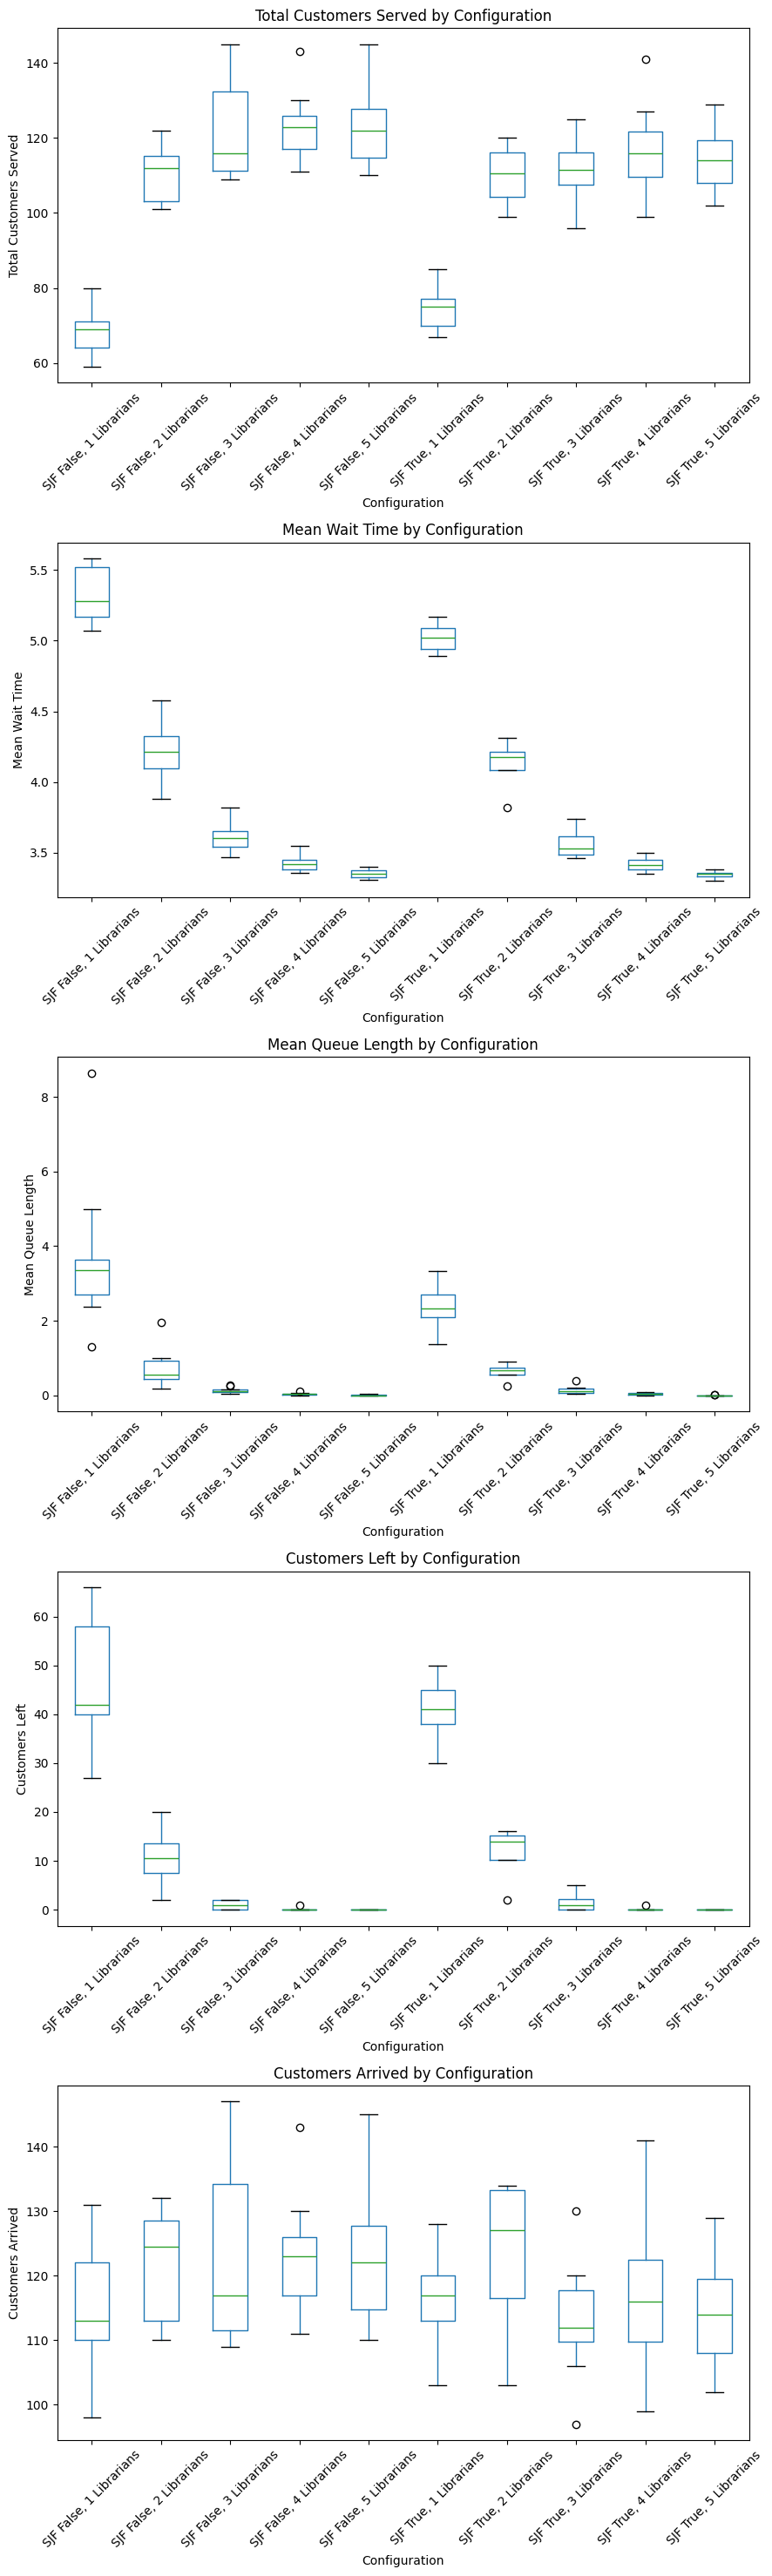
\includegraphics[width=0.7\linewidth]{./boxplot}
	\caption{}
	\label{fig:boxplot}
\end{figure}



\subsection{Hipótesis extraídas de los resultados}
\begin{itemize}
	\item Como puede observarse en la Figura \ref{fig:boxplot} parece haber cierta relación entre la aplicación de la política SJF y la mejora la media de tiempo de espera de los clientes como se sugiere en \cite{modern_operating_systems}
	\item Aparentemente el añadir un quinto bibliotecario no afecta en sentido general las métricas analizadas.
\end{itemize}

\subsection{Experimentos realizados para validar las hipótesis}
Para la primera hipótesis se realizó un análisis de la correlación (ver \ref{fig:heatmap}) de las variables de salida con respecto a la aplicación de la política SJF.

\begin{figure}
	\centering
	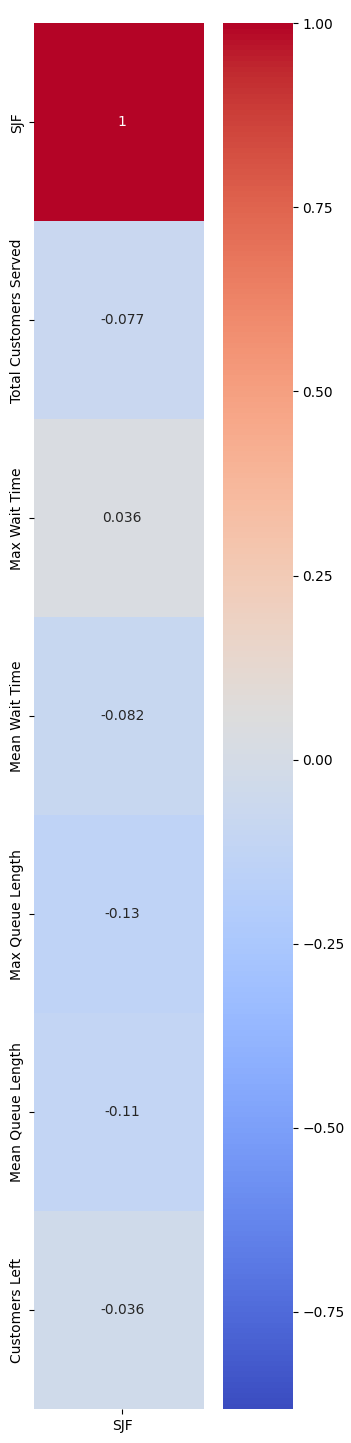
\includegraphics[width=0.7\linewidth]{./heatmap}
	\caption{}
	\label{fig:heatmap}
\end{figure}

 Como puede observarse la aplicación de esta política no tiene correlaciones significativas con ninguna de las variables de salida. \\
Además para comprobar específicamente la relación entre las variables SJF y Mean Wait Time se utilizó una prueba  Mann-Whitney U la cual es una alternativa a la prueba t de Student cuando no se cumplen los supuestos de normalidad. La misma arrojó los resultados siguientes:\\
Mann-Whitney U Test Result: MannwhitneyuResult(statistic=1099.0, pvalue=0.236) \\
El valor p es 0.236, que es mayor que 0.05. Esto indica que no hay suficiente evidencia para rechazar la hipótesis nula. En otras palabras, no hay una diferencia significativa en el tiempo medio de espera (Mean Wait Time) entre las políticas de SJF y FIFO.\\
\\
La Figura \ref{fig:boxplot} indica que al añadir un quinto bibliotecario los datos tienen un comportamiento similar al que tenian con 4. Esto significa que solo representaría un costo adicional a la biblioteca y objetivamente no es necesario. Para validar esta hipótesis se realizó una prueba t de Student (ya que se pudo verificar que se cumplían los supuestos de la misma) para comprobar si existe una diferencia significativa en la cantidad de clientes atendidos en las configuraciones de 4 y 5 bibliotecarios\\
Los resultados fueron:\\
T-test Result: (statistic=0.331, pvalue=0.742, df=45.0)\\
\\
El pvalue es mayor que 0.05 por lo cual podemos concluir que no existe diferencia significativa en la cantidad de clientes atendidos en los grupos de datos de 4 y 5 bibliotecarios, lo cual sugiere que la adición de un quinto bibliotecario no mejora significativamente el servicio en la biblioteca y por lo tanto no es necesario.



\subsection{Análisis de Parada de la Simulación}

\subsubsection{Criterios de Parada}

La elección del momento exacto para detener una simulación es crítica, ya que puede influir significativamente en los resultados obtenidos.

Para establecer el criterio de parada, se utilizó la desviación estándar de las observaciones dividida por la raíz cuadrada del número de observaciones. Este método asegura que los resultados de la simulación sean precisos y estables antes de detener la ejecución. 

\subsubsection{Implementación del Criterio de Parada}

Durante la ejecución de la simulación, se calculó la media y la desviación estándar del número total de clientes que arriban a la biblioteca después de cada iteración. La simulación continuó ejecutándose hasta que la desviación estándar relativa (calculada como la desviación estándar dividida por la raíz cuadrada del número de observaciones y por la media) fue menor que el umbral de convergencia especificado. Se garantiza hacer al menos 100 iteraciones para evitar que la simulación se detenga prematuramente.

% ************************************************************
% ******************* CAPITULO 4 ***************************
% ************************************************************


\section{Modelo Matemático}

\subsection{Descripción del modelo}

El sistema de cuatro bilbiotecarios con política FIFO se basa en un modelo matemático de un sistema de colas con cuatro servidores en paralelo. En este sistema, los clientes llegan siguiendo un proceso de Poisson con una tasa de llegada $\lambda$, y los tiempos de servicio son variables aleatorias exponenciales con tasa $\mu$. Los servidores operan en paralelo, lo que significa que pueden atender a varios clientes simultáneamente.

Este tipo de sistema es conocido como un modelo $M/M/4$ en la teoría de colas, donde:

\begin{itemize}
	\item $M$ denota que los tiempos entre llegadas siguen una distribución de Poisson.
	\item $M$ denota que los tiempos de servicio siguen una distribución exponencial.
	\item 4 indica que hay cuatro servidores en paralelo.
\end{itemize}

El objetivo del modelo es analizar el tiempo promedio de espera en la cola, la probabilidad de que un cliente tenga que esperar para ser atendido, y la utilización de los servidores.

\subsection{Supuestos y restricciones}

El modelo $M/M/4$,se basa en los siguientes supuestos y restricciones:

\begin{enumerate}
	\item \textbf{Proceso de Llegada}: Los clientes llegan de acuerdo a un proceso de Poisson con tasa $\lambda$. Esto implica que las llegadas son independientes y el tiempo entre llegadas sigue una distribución exponencial.
	\item \textbf{Tiempo de Servicio}: Los tiempos de servicio de los servidores son variables aleatorias exponenciales con tasa $\mu$. Esto asegura que la duración del servicio es independiente del tiempo transcurrido.
	\item \textbf{Capacidad de la Cola}: Se asume que la cola tiene capacidad infinita, es decir, no hay límite en el número de clientes que pueden esperar en la cola.
	\item \textbf{Disciplina de la Cola}: Los clientes son atendidos en el orden de llegada (FIFO - First In, First Out).
	\item \textbf{Independencia}: Se asume que los tiempos de llegada y servicio son independientes entre sí y no varían con el tiempo.
	\item \textbf{Servidores Idénticos}: Los cuatro servidores son idénticos en términos de capacidad y eficiencia, es decir, ambos tienen la misma tasa de servicio $\mu$.
\end{enumerate}

\subsection{Comparación de los resultados obtenidos}

Para evaluar la efectividad del modelo, se comparan los resultados obtenidos de las simulaciones con los resultados teóricos esperados del modelo $M/M/4$. Los principales indicadores a considerar incluyen:

\begin{itemize}
	\item \textbf{Número Promedio de Clientes en la Cola ($L_q$)}:
	\begin{itemize}
		\item \textbf{Teórico}: $L_q = 0.001768$ clientes
		\item \textbf{Simulación (FIFO)}: $0.036$ clientes
		\item \textbf{Simulación (SJF)}: $0.036$ clientes
	\end{itemize}
	\item \textbf{Tiempo Promedio de Espera en la Cola ($W_q$)}:
	\begin{itemize}
		\item \textbf{Teórico}: $W_q = 0.000118$ minutos
		\item \textbf{Simulación (FIFO)}: $3.423$ minutos
		\item \textbf{Simulación (SJF)}: $3.418$ minutos
	\end{itemize}
\end{itemize}

Los resultados teóricos y de simulación muestran diferencias significativas respecto al tiempo promedio de espera en la cola. Sin embargo, en la simulación, los tiempos de espera son mayores, esto puede deberse a que los cálculos se realizaron asumiendo que todos los clientes son del tipo Rápido.

Estos resultados resaltan la importancia de considerar tanto el análisis teórico como las simulaciones prácticas para una evaluación completa del rendimiento del sistema.

\subsection{Cálculo de los Valores Teóricos}

Los valores teóricos para el modelo $M/M/4$ se calcularon utilizando las siguientes fórmulas de la teoría de colas de acuerdo a \cite{teoria_de_colas}:

\begin{itemize}
	\item \textbf{Probabilidad de que no haya clientes en el sistema ($P_0$)}:
	\[
	P_0 = \left( \sum_{n=0}^{c-1} \frac{(r^n)}{n!} + \frac{r^c}{c!(1-\rho)} \right)^{-1}
	\]
	Donde $r = \frac{\lambda}{\mu}$ y $\rho = \frac{r}{c}$.
	\item \textbf{Número promedio de clientes en la cola ($L_q$)}:
	\[
	L_q = \frac{r^c \rho}{c!(1-\rho)^2} P_0
	\]
	\item \textbf{Tiempo promedio de espera en la cola ($W_q$)}:
	\[
	W_q = \frac{L_q}{\lambda}
	\]
\end{itemize}

Estos cálculos proporcionan una base teórica para comparar los resultados obtenidos en la simulación y evaluar el rendimiento del sistema de colas bajo diferentes condiciones y políticas de programación.

\section{Conclusiones}

El estudio analizó el rendimiento de una biblioteca mediante la simulación de políticas de atención y variaciones en el número de bibliotecarios. Las pruebas estadísticas mostraron que no existen diferencias significativas entre las políticas FIFO y SJF en el tiempo promedio de espera. Asimismo, se determinó que agregar un quinto bibliotecario no mejora las métricas de rendimiento, representando solo un costo adicional innecesario. El modelo M/M/4 proporcionó una base teórica que, aunque mostró diferencias con los resultados simulados, resaltó la importancia del análisis práctico. Los criterios de parada basados en la desviación estándar garantizaron la precisión de los resultados. Se recomienda no implementar un quinto bibliotecario y considerar la política SJF en contextos específicos. Este estudio combina simulación y análisis teórico para una evaluación integral del sistema.


\begin{thebibliography}{9}
	
	\bibitem{teoria_de_colas}
	García Sabater, J. P. (2015). \textit{Teoría de Colas: Aplicando Teoría de Colas en Dirección de Operaciones}. Grupo ROGLE, Departamento de Organización de Empresas, Universidad Politécnica de Valencia.
	\bibitem{modern_operating_systems}
	Tanenbaum, A. S., \& Bos, H. (2014). \textit{Modern Operating Systems} (4th ed.). Vrije Universiteit, Amsterdam, The Netherlands.
	
	
\end{thebibliography}


\end{document}
